\section{Individual Simulation}~\label{sec:indi}
% \begin{table*}[!htp]
	\aboverulesep0pt
	\belowrulesep0pt
	\extrarowheight1pt
	\centering
	\footnotesize
	\tabcolsep3pt
	\begin{tabularx}{\linewidth}{c|>{\centering\arraybackslash}X|c|c|c|c|>{\centering\arraybackslash}m{8em}}
		\toprule
        \multirow[m]{2}{*}{\textbf{Objectives}} 
		& \multirow[m]{2.5}{2.5em}{\textbf{Paper}} & \multicolumn{4}{c|}{\textbf{Aritecture}} & \multirow[m]{2.5}{*}{\textbf{Construtction}} \\
		\cmidrule{3-6}
		&  & \textbf{Profile} & \textbf{Memory} & \textbf{Planning} & \textbf{Action Domain} &  \\
		\midrule
		\multirow[m]{19}{*}{\textbf{Characters}} & \cite{brahman2021letcharacterstellstory} & Dialogue/Description & Short-term & - & Open/Closed  & Parametric  \\
		\cmidrule{2-7}
		& \cite{chen2023largelanguagemodelsmeet} & Dialogue/Description & Short-term & - & Open  & \multicolumn{1}{m{7em}}{Parametric /Nonparametric }\\
		\cmidrule{2-7}
		& \cite{schwitzgebel2023creatinglargelanguagemodel} & Dialogue & Short-term & - & Open  & Parametric  \\
		\cmidrule{2-7}
		& \cite{park2023generativeagentsinteractivesimulacra} & Description & Short/Long-term & Interactive & Open  & Nonparametric  \\
		\cmidrule{2-7}
		& \cite{agrawal-etal-2023-multimodal} & Dialogue/Description & Short-term & - & Open  & Parametric  \\
		\cmidrule{2-7}
		& \cite{li2023chatharuhirevivinganimecharacter} & Dialogue & Short-term & Isolated & Open  & Parametric  \\
		\cmidrule{2-7}
		& \cite{gao2023livechatlargescalepersonalizeddialogue} & Dialogue/Description & Short/Long-term & - & Open/Closed  & Parametric  \\
		\cmidrule{2-7}
		& \cite{wang2024rolellmbenchmarkingelicitingenhancing} & Description/Dialogue & Short-term & - & Open/Closed  & Parametric  \\
		\cmidrule{2-7}
		& \cite{shao2023characterllmtrainableagentroleplaying} & Description & Short-term & - & Open  & Parametric  \\
		\cmidrule{2-7}
		& \cite{wang2024incharacterevaluatingpersonalityfidelity} & - & Short-term & - & Open/Closed  & - \\
		\cmidrule{2-7}
		& \cite{zhou2023characterglmcustomizingchineseconversational} & Description/Dialogue & Short-term & - & Open  & Parametric  \\
		\cmidrule{2-7}
		& \cite{shen2024roleevalbilingualroleevaluation} & Description & Short-term & - & Closed  & Parametric  \\
		\cmidrule{2-7}
		& \cite{tu2024characterevalchinesebenchmarkroleplaying} & Dialogue & Short-term & - & Open  & Nonparametric  \\
		\cmidrule{2-7}
		& \cite{yu2024neekoleveragingdynamiclora} & Description & Short-term & - & Open  & Parametric  \\
		\cmidrule{2-7}
		& \cite{xu2024characterdestinylargelanguage} & Description & Short/Long-term & - & Closed  & Nonparametric  \\
		\cmidrule{2-7}
		& \cite{yuan2024evaluatingcharacterunderstandinglarge} & Description & Short-term & - & Open/Closed  & Nonparametric  \\
		\cmidrule{2-7}
		& \cite{ran2024capturingmindsjustwords} & Description/Dialogue & Short/Long-term & - & Open/Closed  & Parametric  \\
		\cmidrule{2-7}
		& \cite{dai2024mmrolecomprehensiveframeworkdeveloping} & Description & Short-term & - & Open  & Parametric  \\
		\cmidrule{2-7}
		& \cite{yu2024dialogueprofiledialoguealignmentframework} & Dialogue & Short-term & - & Open  & Parametric  \\
		\midrule
		 \multirow[m]{35}{6em}{\textbf{Demographics}}& \cite{karra2023estimatingpersonalitywhiteboxlanguage} & Dialogue/Description & Short-term & - & Closed  & Parametric  \\
		 \cmidrule{2-7}
		& \cite{jiang2023evaluatinginducingpersonalitypretrained} & Description & Short-term & - & Closed  & Nonparametric  \\
		\cmidrule{2-7}
		& \cite{Liu_2022} & Description & Short/Long-term & - & Open  & Parametric  \\
		\cmidrule{2-7}
		& \cite{Argyle_2023} & Description & Short-term & - & Open  & Nonparametric  \\
		\cmidrule{2-7}
		& \cite{horton2023largelanguagemodelssimulated} & Description & Short-term & - & Closed  & Nonparametric  \\
		\cmidrule{2-7}
		& \cite{xie2023wallstreetneophytezeroshot} & Description & Short-term & Isolated & Closed  & Nonparametric  \\
		\cmidrule{2-7}
		& \cite{deshpande2023toxicitychatgptanalyzingpersonaassigned} & Description & Short-term & - & Open  & Nonparametric  \\
		\cmidrule{2-7}
		& \cite{xiang2023languagemodelsmeetworld} & Description & Short-term & Interactive & Open  & Parametric  \\
		\cmidrule{2-7}
		& \cite{song2023largelanguagemodelsdeveloped} & Description & Short-term & - & Closed  & Nonparametric  \\
		\cmidrule{2-7}
		& \cite{cheng2023markedpersonasusingnatural} & Description & Short-term & - & Open  & Nonparametric  \\
		\cmidrule{2-7}
		& \cite{wang2024userbehaviorsimulationlarge} & Description & Short/Long-term & - & Open  & Nonparametric  \\
		\cmidrule{2-7}
		& \cite{serapiogarcía2023personalitytraitslargelanguage} & Description & Short-term & - & Open  & Nonparametric  \\
		\cmidrule{2-7}
		& \cite{huang2024emotionallynumbempatheticevaluating} & Description & Short-term & - & Closed  & Nonparametric  \\
		\cmidrule{2-7}
		& \cite{tu2023characterchatlearningconversationalai} & Description & Short/Long-term & - & Open  & Nonparametric  \\
		\cmidrule{2-7}
		& \cite{abbasian2024conversationalhealthagentspersonalized} & Description & Short/Long-term & Interactive & Open  & Nonparametric  \\
		\cmidrule{2-7}
		& \cite{chen2024moneymouthisevaluating} & Description & Short/Long-term & Interactive & Closed  & Nonparametric  \\
		\cmidrule{2-7}
		& \cite{li2024econagentlargelanguagemodelempowered} & Description & Short/Long-term & - & Open  & Nonparamaetric  \\
		\cmidrule{2-7}
		& \cite{shea2023buildingpersonaconsistentdialogue} & Dialogue & Short-term & - & Open  & Parametric  \\
		\cmidrule{2-7}
		& \cite{chawla2023selfishwiselyinvestigatingimpact} & Dialogue & Short-term & - & Open  & Parametric  \\
		\cmidrule{2-7}
		& \cite{10.19066/COGSCI.2024.35.1.002} & - & Short-term & Interactive & Open  & Nonparametric  \\
		\cmidrule{2-7}
		& \cite{gupta2024biasrunsdeepimplicit} & Description & Short-term & - & Open  & Nonparametric  \\
		\cmidrule{2-7}
		& \cite{li2024steerabilitylargelanguagemodels} & Dialogue & Short-term & - & Open  & Parametric  \\
		\cmidrule{2-7}
		& \cite{huang2024embodiedgeneralistagent3d} & Description & Short-term & Isolated & Open  & Parametric  \\
		\cmidrule{2-7}
		& \cite{xie2024largelanguagemodelagents} & Description & Short-term &  & Closed  & Nonparametric  \\
		\cmidrule{2-7}
		& \cite{Lee_2024} & Description & Short-term & - & Closed  & Nonparametric  \\
		\cmidrule{2-7}
		& \cite{li2024culturellmincorporatingculturaldifferences} & Dialogue & Short-term & - & Open  & Parametric  \\
		\cmidrule{2-7}
		& \cite{weng2024controllmcraftingdiversepersonalities} & - & Short/Long-term & - & Open  & Nonparamatric  \\
		\cmidrule{2-7}
		& \cite{sun2024randomsiliconsamplingsimulating} & Description & Short-term & - & Closed  & Nonparametric  \\
		\cmidrule{2-7}
		& \cite{Bisbee_Clinton_Dorff_Kenkel_Larson_2024} & Description & Short-term & - & Closed  & Nonparametric  \\
		\cmidrule{2-7}
		& \cite{ge2024scalingsyntheticdatacreation} & Description & Short-term & - & Open  & Parametric  \\
		\cmidrule{2-7}
		& \cite{Qu2024PerformanceAB} & Description & Short-term & - & Closed  & Nonparametric  \\
		\cmidrule{2-7}
		& \cite{qiu2024interactiveagentssimulatingcounselorclient} & Description & Short-term & - & Open  & Nonparametric  \\
		\bottomrule
	\end{tabularx}
    \caption{A list of representative works of individual simulation}
\end{table*}


\begin{table*}[!htp]
\aboverulesep0pt
\belowrulesep0pt
\extrarowheight1pt
\centering
\footnotesize
\tabcolsep3pt
\resizebox*{!}{\dimexpr\textheight-3\baselineskip\relax}{\begin{tabularx}{\linewidth}{c|>{\centering\arraybackslash}X|c|c|c|c|>{\centering\arraybackslash}m{8em}}
    \toprule
    \multirow[m]{2}{*}{\textbf{Objectives}} 
    & \multirow[m]{2.5}{2.5em}{\textbf{Paper}} & \multicolumn{4}{c|}{\textbf{Aritecture}} & \multirow[m]{2.5}{*}{\textbf{Construtction}} \\
    \cmidrule{3-6}
    &  & \textbf{Profile} & \textbf{Memory} & \textbf{Planning} & \textbf{Action Domain} &  \\
    \midrule
    \multirow[m]{19}{*}{\textbf{Characters}} & 
    Brahman et al.
    \cite{brahman2021letcharacterstellstory} & Dialogue/Description & Short-term & - & Open/Closed  & Parametric  \\
    \cmidrule{2-7}
    & Chen et al. \cite{chen2023largelanguagemodelsmeet} & Dialogue/Description & Short-term & - & Open  & \multicolumn{1}{m{7em}}{Parametric /Nonparametric }\\
    \cmidrule{2-7}
    & Schwitzgebel et al. \cite{schwitzgebel2023creatinglargelanguagemodel} & Dialogue & Short-term & - & Open  & Parametric  \\
    \cmidrule{2-7}
    & Generative Agents \cite{park2023generativeagentsinteractivesimulacra} & Description & Short/Long-term & - & Open  & Nonparametric  \\
    \cmidrule{2-7}
    & Agrawal et al. \cite{agrawal-etal-2023-multimodal} & Dialogue/Description & Short-term & - & Open  & Parametric  \\
    \cmidrule{2-7}
    & ChatHaruhi \cite{li2023chatharuhirevivinganimecharacter} & Dialogue & Short-term & - & Open  & Parametric  \\
    \cmidrule{2-7}
    & LiveChat \cite{gao2023livechatlargescalepersonalizeddialogue} & Dialogue/Description & Short/Long-term & - & Open/Closed  & Parametric  \\
    \cmidrule{2-7}
    & RoleLLM \cite{wang2024rolellmbenchmarkingelicitingenhancing} & Description/Dialogue & Short-term & - & Open/Closed  & Parametric  \\
    \cmidrule{2-7}
    & CharacterLLM \cite{shao2023characterllmtrainableagentroleplaying} & Description & Short-term & Subjective & Open  & Parametric  \\
    \cmidrule{2-7}
    & InCharacter \cite{wang2024incharacterevaluatingpersonalityfidelity} & - & Short-term & - & Open/Closed  & - \\
    \cmidrule{2-7}
    & CharacterGLM \cite{zhou2023characterglmcustomizingchineseconversational} & Description/Dialogue & Short-term & - & Open  & Parametric  \\
    \cmidrule{2-7}
    & RoleEval \cite{shen2024roleevalbilingualroleevaluation} & Description & Short-term & - & Closed  & Parametric  \\
    \cmidrule{2-7}
    & CharacterEval \cite{tu2024characterevalchinesebenchmarkroleplaying} & Dialogue & Short-term & - & Open  & Nonparametric  \\
    \cmidrule{2-7}
    & Neeko \cite{yu2024neekoleveragingdynamiclora} & Description & Short-term & - & Open  & Parametric  \\
    \cmidrule{2-7}
    & Character is Destiny \cite{xu2024characterdestinylargelanguage} & Description & Short/Long-term & - & Closed  & Nonparametric  \\
    \cmidrule{2-7}
    & Yuan et al. \cite{yuan2024evaluatingcharacterunderstandinglarge} & Description & Short-term & - & Open/Closed  & Nonparametric  \\
    \cmidrule{2-7}
    & Capturing Minds \cite{ran2024capturingmindsjustwords} & Description/Dialogue & Short/Long-term & Subjective & Open/Closed  & Parametric  \\
    \cmidrule{2-7}
    & MMRole \cite{dai2024mmrolecomprehensiveframeworkdeveloping} & Description & Short-term & - & Open  & Parametric  \\
    \cmidrule{2-7}
    & Yu et al. \cite{yu2024dialogueprofiledialoguealignmentframework} & Dialogue & Short-term & - & Open  & Parametric  \\
    \cmidrule{2-7}
    & Rational sensibility \cite{sun2023rational} & - & Short-term & Empathetic & Closed & Parametric \\
    \midrule
     \multirow[m]{35}{6em}{\textbf{Demographics}}& Karra et al.\cite{karra2023estimatingpersonalitywhiteboxlanguage} & Dialogue/Description & Short-term & - & Closed  & Parametric  \\
     \cmidrule{2-7}
    & Jiang et al. \cite{jiang2023evaluatinginducingpersonalitypretrained} & Description & Short-term & - & Closed  & Nonparametric  \\
    \cmidrule{2-7}
    & Liu et al. \cite{Liu_2022} & Description & Short/Long-term & - & Open  & Parametric  \\
    \cmidrule{2-7}
    & Out of One, Many \cite{Argyle_2023} & Description & Short-term & - & Open  & Nonparametric  \\
    \cmidrule{2-7}
    & Simulated Economic Agents \cite{horton2023largelanguagemodelssimulated} & Description & Short-term & - & Closed  & Nonparametric  \\
    \cmidrule{2-7}
    & The wall street neophyte \cite{xie2023wallstreetneophytezeroshot} & Description & Short-term & Empathetic & Closed  & Nonparametric  \\
    \cmidrule{2-7}
    & Toxicity in ChatGPT \cite{deshpande2023toxicitychatgptanalyzingpersonaassigned} & Description & Short-term & - & Open  & Nonparametric  \\
    \cmidrule{2-7}
    & Song et al. \cite{song2023largelanguagemodelsdeveloped} & Description & Short-term & - & Closed  & Nonparametric  \\
    \cmidrule{2-7}
    & Marked Personas \cite{cheng2023markedpersonasusingnatural} & Description & Short-term & - & Open  & Nonparametric  \\
    \cmidrule{2-7}
    & Wang et al. \cite{wang2024userbehaviorsimulationlarge} & Description & Short/Long-term & - & Open  & Nonparametric  \\
    \cmidrule{2-7}
    & Serapio-García et al. \cite{serapiogarcía2023personalitytraitslargelanguage} & Description & Short-term & - & Open  & Nonparametric  \\
    \cmidrule{2-7}
    & Huang et al. \cite{huang2024emotionallynumbempatheticevaluating} & Description & Short-term & - & Closed  & Nonparametric  \\
    \cmidrule{2-7}
    & CharacterChat \cite{tu2023characterchatlearningconversationalai} & Description & Short/Long-term & - & Open  & Nonparametric  \\
    \cmidrule{2-7}
    & Conversational health agents \cite{abbasian2024conversationalhealthagentspersonalized} & Description & Short/Long-term & Empathetic & Open  & Nonparametric  \\
    \cmidrule{2-7}
    & Chen et al. \cite{chen2024moneymouthisevaluating} & Description & Short/Long-term & - & Closed  & Nonparametric  \\
    \cmidrule{2-7}
    & EconAgent \cite{li2024econagentlargelanguagemodelempowered} & Description & Short/Long-term & - & Open  & Nonparamaetric  \\
    \cmidrule{2-7}
    & Shea et al. \cite{shea2023buildingpersonaconsistentdialogue} & Dialogue & Short-term & - & Open  & Parametric  \\
    \cmidrule{2-7}
    & Be Selfish, But Wisely \cite{chawla2023selfishwiselyinvestigatingimpact} & Dialogue & Short-term & - & Open  & Parametric  \\
    \cmidrule{2-7}
    & Chain of Empathy \cite{10.19066/COGSCI.2024.35.1.002} & - & Short-term & Empathetic & Open  & Nonparametric  \\
    \cmidrule{2-7}
    & Bias Runs Deep \cite{gupta2024biasrunsdeepimplicit} & Description & Short-term & - & Open  & Nonparametric  \\
    \cmidrule{2-7}
    & Li et al. \cite{li2024steerabilitylargelanguagemodels} & Dialogue & Short-term & - & Open  & Parametric  \\
    \cmidrule{2-7}
    & Xie et al. \cite{xie2024largelanguagemodelagents} & Description & Short-term & Subjective & Closed  & Nonparametric  \\
    \cmidrule{2-7}
    & Lee et al. \cite{Lee_2024} & Description & Short-term & - & Closed  & Nonparametric  \\
    \cmidrule{2-7}
    & CultureLLM \cite{li2024culturellmincorporatingculturaldifferences} & Dialogue & Short-term & - & Open  & Parametric  \\
    \cmidrule{2-7}
    & ControlLM \cite{weng2024controllmcraftingdiversepersonalities} & - & Short/Long-term & - & Open  & Nonparamatric  \\
    \cmidrule{2-7}
    & Random Silicon Sampling \cite{sun2024randomsiliconsamplingsimulating} & Description & Short-term & - & Closed  & Nonparametric  \\
    \cmidrule{2-7}
    & Bisbee et al. \cite{Bisbee_Clinton_Dorff_Kenkel_Larson_2024} & Description & Short-term & - & Closed  & Nonparametric  \\
    \cmidrule{2-7}
    & PersonaHub \cite{ge2024scalingsyntheticdatacreation} & Description & Short-term & - & Open  & Parametric  \\
    \cmidrule{2-7}
    & Qu et al. \cite{Qu2024PerformanceAB} & Description & Short-term & - & Closed  & Nonparametric  \\
    \cmidrule{2-7}
    & Interactive Agents \cite{qiu2024interactiveagentssimulatingcounselorclient} & Description & Short-term & - & Open  & Nonparametric  \\
    \bottomrule
\end{tabularx}}
\caption{A list of representative works of individual simulation.}
\label{tab:indi}
\end{table*}
% For a long time, scientists have focused on studying individual behavior. The Stanford Prison Experiment, for instance, explored how a person’s character changed in extreme environments, while the Obedience to Authority Study examined the capacity of individuals to resist immoral authority. Nowadays, LLMs are increasingly used to simulate the behavior of specific individuals. Across a broad range of experiments, individual simulation can be defined as the use of LLMs to replicate the behaviors of specific individuals. Researchers train and prompt LLMs with individualized data, guiding them to respond with specific actions in given situations.This new approach allows researchers to replicate individual behaviors without the ethical concerns associated with direct human experiments, helping to address moral issues in social science research. Furthermore, individual simulation using LLMs enhances interactions between the models and users, opening up new opportunities for their application. To successfully create individual simulations, key elements such as simulation model architecture, model construction methods, individual objectives, and evaluation strategies must be thoroughly understood and integrated.\XY{Reformulate this paragraph: (1) Previous studies on individual social behavior were based on questionnaires, interviews etc... (2) Then transit to the recent use of LLMs in ... (what is individual simulation, how to implement) (3) The key components of individual simulation is ... Note: before introducing the advantages of LLM-based simulation, you need to first explain what is individual simulation. The description of different stages can be moved to the trend section.}

% Traditionally, research on individual behavior has relied on methods such as questionnaires~\cite{granovetter1973strength,katz2015social} and interviews~\cite{gubrium2002individual,roulston2003learning}. While these methods provide highly authentic and detailed data, they are costly, challenging to scale, and may involve ethical concerns. 
% \slb{I think we should not start from the study of individual behavior.} \XN{agree, revised. BTW, the citation style using (names, year) format influences the readability of the paper dramatically. Can we use the numerical citation style?}
% Recently, with the demonstrated capability of LLMs in generating natural language, a series of studies~\cite{park2023generative,shao2023characterllmtrainableagentroleplaying,wang2023rolellm} has explored using LLMs as agents to simulate human behaviors, yielding significant progress in individual simulation.

Individual simulation focuses on designing a modular architecture that integrates individualized data for the construction of agents and simulating the specific objective with high fidelity.
In this section, we first outline the basic architecture of the agent in the individual simulation with four key components in~\S\ref{subsec:indi_arch}. Then, two construction methods are discussed in~\S\ref{subsec:indi_cons} to implement the integration of individualized data into objectives introduced in~\S\ref{subsec:indi_obj}. The evaluation methods are examined from different perspectives in~\S\ref{subsec:indi_eval}. The overall framework is presented in Figure~\ref{fig:fm_indi} and representative works are summarized in Table~\ref{tab:indi}.

% Next, to better integrate individualized data into agents, we delve into the construction of agents in the individual simulation. Built upon these foundations, we explore the diverse simulation objectives that individual simulation seeks to achieve. Finally, we examine the evaluation methods in individual simulation from various perspectives. The overall framework is presented in Figure~\ref{fig:fm_indi}.


\subsection{Architecture}\label{subsec:indi_arch}
% In the context of agent-based LLMs, architecture refers to the modular structure that enhances the performance of individual simulations. While the components of these architectures may vary based on specific tasks or situations, they typically share several core elements: profile, memory, planning, and action. In summary, the profile system defines the agent's identity, the memory system improves performance by providing relevant context, the planning system organizes solutions to tasks, and the action system interacts directly with the environment and users.
To effectively accomplish individual simulation, it is essential to construct an agent architecture that can accurately replicate the features of the individual. This requires a balance between theoretical abstraction and practical implementation to capture the complexity of human behaviors. Typically, this architecture is modularized into four core components: \textbf{profile}, \textbf{memory}, \textbf{planning}, and \textbf{action}.



\subsubsection{Profile}

Profile differentiates the unique characteristics of simulated individuals, encompassing attributes, behaviors, and constraints. The profiles differ in the ways of construction and their forms.

\paragraph{Profile Construction}


Profile construction refers to the process of collecting individual-related information, which can be categorized into \textit{manual modification} and \textit{LLM generation}. 
\textit{{\ul Manual modification}} takes advantage of publicly available data to create high-quality profiles through a human-guided process. According to the collected sources, manual modification can also be classified into three categories:  handcrafting, online communities, and historical works. Handcrafting manually organized some coarse strength information, such as well-known characters~\cite{wang2023humanoidagentsplatformsimulating} and specific personalities~\cite{deshpande2023toxicitychatgptanalyzingpersonaassigned,cheng2023markedpersonasusingnatural}, while online communities construct profiles built on the web data like Wikipedia~\cite{shao2023characterllmtrainableagentroleplaying} and social media~\cite{gao2023livechatlargescalepersonalizeddialogue}, where the profile implicitly exists in conversations and materials.
In addition, literary works serve as additional descriptions that reflect the author's thoughts~\cite{schwitzgebel2023creatinglargelanguagemodel} and characters in the storyline~\cite{brahman2021letcharacterstellstory,li2023chatharuhirevivinganimecharacter}. 
\textit{{\ul LLM generation}} automatically generates the expected persona-based information profiles by prompting LLMs with essential individual details~\cite{tu2023characterchatlearningconversationalai,wang2024rolellmbenchmarkingelicitingenhancing,wang2024incharacterevaluatingpersonalityfidelity}. This method explores diverse profiles with ease, while the quality needs human supervision with caution.

% \slb{Emphasize the characteristics of different methods and organize this paragraph using the differences and connections between the three types of methods.}

\paragraph{Profile Form}


Profile form defines the format of individual information, which can be categorized into  \textit{descriptions} and \textit{conversations}.
\textit{{\ul Descriptions}} directly describe basic individual information or identity with details like name, age, and gender~\cite{jang2022customizedconversationcustomizedconversation,wang2023humanoidagentsplatformsimulating}. While descriptions can intuitively reflect the basic attributes of an individual, deeper contextual information can also be ignored.
On the contrary, \textit{{\ul conversations}} implicitly reflect the character profile through dialogue.
A substantial amount of conversational data is derived from sources such as films, literary works, and scripts~\cite{li2021dialoguehistorymatterspersonalized,brahman2021letcharacterstellstory,jandaghi2023faithfulpersonabasedconversationaldataset,yu2024dialogueprofiledialoguealignmentframework}. 
Considering the extensive commonsense knowledge learned by LLMs in the pre-training stage, recent works leverage LLMs to generate individual dialogues~\cite{li2023chatharuhirevivinganimecharacter,ge2024scalingsyntheticdatacreation}, which defines the artistic genre through six essential elements to generate detailed drama scripts~\cite{wu2024roleplaydramainteractionllmsolution} and imitates speaking styles through context learning~\cite{wang2024rolellmbenchmarkingelicitingenhancing,yu2024neekoleveragingdynamiclora}.

% For instance, ~\cite{wu2024roleplaydramainteractionllmsolution} defines the artistic genre through six essential elements, with a pipeline that employs LLMs to transform publicly available stories from the web into detailed drama scripts.Meanwhile,~\cite{wang2024rolellmbenchmarkingelicitingenhancing,yu2024neekoleveragingdynamiclora} allow LLMs to imitate speaking styles through context learning.

\subsubsection{Memory}
Memory is designed to store perceived or generated information, helping agents maintain consistency and continuity of behavior and overcome the limited context window of LLMs. Considering the complexity of memory, researchers struggle to design more efficient memory types and operations.

\paragraph{Memory Type}
Based on the temporal span of stored content, memory can be commonly divided into two types, namely \textit{short-term memory} and \textit{long-term memory}. \textit{{\ul Short-term memory}} records the instant local information that the agent perceives, which can be further divided into simulation contents and simulation supplements. Simulation contents include essential interaction data like user instructions~\cite{schwitzgebel2023creatinglargelanguagemodel,deshpande2023toxicitychatgptanalyzingpersonaassigned}, dialogue history~\cite{xiang2023languagemodelsmeetworld,huang2024embodiedgeneralistagent3d}, and user/environment responses~\cite{xie2023wallstreetneophytezeroshot}. Simulation supplements provide additional environmental information including scene descriptions~\cite{xie2023wallstreetneophytezeroshot,agrawal-etal-2023-multimodal} and scene-related experiences~\cite{shao2023characterllmtrainableagentroleplaying,xu2024characterdestinylargelanguage}, which navigate agents through the simulation to perform tasks appropriately.
\textit{{\ul Long-term memory}} stores persistent global information, preventing deviations from intended goals, which holds extensive individual-specific information stably, including past experiences and behaviors, current knowledge, and skills~\cite{li2024econagentlargelanguagemodelempowered,xu2024characterdestinylargelanguage}. With the proposal of using the vector database as the long-term memory hub, the management, retrieval, and organization of memory is more effective~\cite{lin2023agentsimsopensourcesandboxlarge}.

\paragraph{Memory Operation}

Memory operations stand for the continuous updating and utilization of memory by the agent. The common memory operations include three types, namely \textit{memory writing}, \textit{memory retrieval}, and \textit{memory reflection}.

\textit{{\ul Memory writing}} aims to incorporate the relevant historical content into the memory. This process mirrors human memory formation, where useful information is retained for future retrieval. The memories to be written vary from user-specific dialogue history~\cite{li2021dialoguehistorymatterspersonalized}, new skills~\cite{wang2023voyageropenendedembodiedagent}, to selected papers and other forms~\cite{wang2024surveyagentconversationalpersonalizedefficient}.

% For instance, ~\cite{li2021dialoguehistorymatterspersonalized}  incorporates user-specific dialogue history into the response selection. Considering the changing environment,~\cite{wang2023voyageropenendedembodiedagent} adds new skills into the skill library, while~\cite{wang2024surveyagentconversationalpersonalizedefficient} updates selected papers into a target collection.

\textit{{\ul Memory retrieval}} serves to extract valuable content from memory based on customized requirements. The overall performance of the individual simulation highly relies on the effectiveness of memory retrieval since simulations are sensitive to the context.
% Since simulations are context-sensitive, the effectiveness of memory retrieval becomes crucial in determining overall performance. 
Traditional retrieval technologies rely on similarity such as keyword matching~\cite{chen2024socialbenchsocialityevaluationroleplaying} and embedding vectors~\cite{lin2023agentsimsopensourcesandboxlarge}, while recent works introduce the retrieval model to select the most relevant information~\cite{chen2023chatcottoolaugmentedchainofthoughtreasoning,salemi2024lamplargelanguagemodels}.

\textit{{\ul Memory reflection}} mirrors the human ability to reconsider past behaviors and opinions. Specifically, it helps the agent to organize, refine, and elevate memories into more abstract and insightful concepts. Generative Agents~\cite{park2023generativeagentsinteractivesimulacra} maintains a comprehensive record of agents' experiences with a tree-structured reflection process to optimize memory usage. ProAgent~\cite{zhang2024proagentbuildingproactivecooperative} incorporates memory reflection with validation and belief correction to improve the agent’s planning and decision-making. Voyager~\cite{wang2023voyageropenendedembodiedagent} allows agents to reflect on their behavior and update their skill libraries through self-verification. Although the application scenarios of memory reflection are still limited, it shows great improvement in enhancing performance and increasing the depth of simulations, especially in complex environments.



\subsubsection{Planning}

Planning is the process of deciding on a series of actions aimed at achieving specific goals. Traditional planning tasks typically focus on solving particular problems, such as mathematical reasoning~\cite{wang2023plan} or embodied tasks~\cite{wu2023embodied, song2023llmplannerfewshotgroundedplanning}. At the individual simulation level, however, agents are expected to go beyond mere problem-solving. They should also be able to simulate personalized thinking and emotional responses during interactions with specific individuals. This extends planning into two additional categories: empathetic planning and subjective planning.

\paragraph{Empathetic planning} Empathetic planning refers to an agent's ability to infer and perceive the behavior and emotions of others before taking action. It involves using Chain-of-Thought (CoT) reasoning to understand the situations of others and make adaptive decisions or judgments~\cite{xie2023wallstreetneophytezeroshot, 10.19066/COGSCI.2024.35.1.002, sun2023rational}. This allows the agent to tailor its actions based on the emotional and behavioral context, guiding the acquisition of personalized feedback.

\paragraph{Subjective planning} Subjective planning refers to the actions an agent takes based on its own thoughts and feelings, in line with its predefined role or identity.
This can involve utilizing inner monologues from simulated characters to fine-tune LLMs~\cite{shao2023characterllmtrainableagentroleplaying,ran2024capturingmindsjustwords} or using CoT to guide LLMs to express themselves according to their own beliefs~\cite{xie2024largelanguagemodelagents}. 
This form of planning is driven by the agent's internal state, rather than by external stimuli or the needs of others.


\subsubsection{Action}\label{sec:action}

Action refers to the direct interaction between LLMs and their environment. Action encompasses two key aspects: the action situation, which describes the context in which actions occur, and the action domain, which defines the requirements for action space. Action serves as the interface for simulating human behavior, allowing LLMs to execute tasks that mimic real-world actions and responses. This interaction enables a deeper understanding of human-like decision-making and execution in various scenarios.

\paragraph{Action Situation}
With individual simulations focusing on more and more diverse and complicated situations, various action situations spring out accordingly, ranging from dialogue~\cite{cho2022personalizeddialoguegeneratorimplicit}, games~\cite{light2023avalonbenchevaluatingllmsplaying}, real word~\cite{xiang2023languagemodelsmeetworld}, etc. Typically, action situations can be divided into \textit{simple dialogues} and \textit{crafted situations}.

\textit{{\ul Simple dialogues}} are few-turn conversations without restricted environments, such as constructing dialogues between two characters~\cite{brahman2021letcharacterstellstory}. Recent researches utilize simple dialogues to induce potential attributes within the models, involving personality~\cite{karra2023estimatingpersonalitywhiteboxlanguage,jiang2023evaluatinginducingpersonalitypretrained}, traits~\cite{serapiogarcía2023personalitytraitslargelanguage} and toxicity~\cite{deshpande2023toxicitychatgptanalyzingpersonaassigned}. Other works conduct evaluations of persona with interviewing~\cite{wang2024incharacterevaluatingpersonalityfidelity} or questionnaire~\cite{pan2023llmspossesspersonalitymaking} with simple dialogues to facilitate their experiment.

\textit{{\ul Crafted situations}} are elaborately designed environments including detailed rules and surrounding descriptions. Common situations like games are modified from simple dialogues. They leverage game rules to provide a settled virtual topic for both users and agents to play in, especially in the board role-playing games~\cite{light2023avalonbenchevaluatingllmsplaying,light2023avalonbenchevaluatingllmsplaying}~\cite{chalamalasetti2023clembenchusinggameplay}. Besides, researchers have developed a more delicate environment called sandbox~\cite{chen2024socialbenchsocialityevaluationroleplaying}, which not only includes rules but establish an objective environment. To further enrich the individual simulation situation, some authors add some elements existing in scripts like facial expression, tiny movements~\cite{agrawal-etal-2023-multimodal,wu2024roleplaydramainteractionllmsolution}, and nuanced information from environment images~\cite{dai2024mmrolecomprehensiveframeworkdeveloping}.

\paragraph{Action Domain} The Action domain can be commonly divided into \textit{close domain} and \textit{open domain} based on the restriction of action space.
% \slb{Add a sentence for introducing.}

\textit{{\ul Closed domain}} simulation occurs when the available action space is limited. In simple situations such as completing questionnaires testing~\cite{karra2023estimatingpersonalitywhiteboxlanguage}, making decisions from a set of options~\cite{horton2023largelanguagemodelssimulated}, or rating with predefined standards~\cite{wang2024incharacterevaluatingpersonalityfidelity}, the action space of LLMs is determined by researchers ahead of simulation to make responses predictable. In practical scenarios, LLMs are required to choose tools~\cite{chen2023chatcottoolaugmentedchainofthoughtreasoning,yuan2023skill} or select specific functions to complete concrete tasks, like recommending, browsing, and compiling.
% ~\XN{maybe need references here}. 
Individual simulation with agents in closed-domain tasks can improve human work efficiency, extending beyond entertainment purposes.

\textit{{\ul Open domain}} simulation places few restrictions on actions, allowing LLMs to generate responses freely. This approach more closely resembles real-world conditions, but also demands higher standards for individual simulation. Among various open-domain tasks, taking actions through conversation is a popular method for simulating individual behavior~\cite{brahman2021letcharacterstellstory,li2023chatharuhirevivinganimecharacter,zhou2023characterglmcustomizingchineseconversational,yu2024neekoleveragingdynamiclora}, in which the varied settings stimulate LLMs’ potential for individual simulation and allow researchers to oversee simulations across diverse and nuanced dimensions. Another growing method of open-domain simulation is scenario-based interaction, where LLMs are assigned roles and are required to interact in crated situations like sandbox~\cite{wang2023voyageropenendedembodiedagent,lin2023agentsimsopensourcesandboxlarge} or established game settings~\cite{light2023avalonbenchevaluatingllmsplaying,chalamalasetti2023clembenchusinggameplay}.


\subsection{Construction}\label{subsec:indi_cons}

% \slb{Rephrase.}
Construction indicates the process of integrating individual data into the established model of LLMs, which aligns the design model and the individual, thus creating the simulating LLMs. Generally, construction methods are distinguished into two types, namely \textbf{nonparametric prompting} and \textbf{parametric training}.

\subsubsection{Nonparametric Prompting}

Nonparametric prompting, i.e. prompt engineering, is a method of interacting with LLMs by designing and optimizing input prompts. In some individual simulations, the description-based profile is implemented by a system prompt. Researchers often create system prompts that begin with \textit{``You are a..."} to assign models specific demographic features and roles~\cite{deshpande2023toxicitychatgptanalyzingpersonaassigned}. Besides, LLM outputs are enhanced in some works through few-shot prompting by providing specific examples to inject detailed information and improve response quality. Moreover, incorporating problem-specific details directly within prompt structures can significantly enhance the effectiveness of the simulation.

Short-term memory is often implemented by nonparametric prompting. For situation-based individual simulations, environment descriptions and behavior rules are typically conveyed through prompt engineering~\cite{chalamalasetti2023clembenchusinggameplay}. Since situational information is generally objective and must be followed, emphasizing this information directly in the input is a rather effective method for constructing simulations. However, due to the context window limitations of LLMs, the quality of the profile prompt significantly restricts prompt-based individual simulations. 
Moreover, the preset template configurations as the \textit{``assistant"} within 
LLMs pose a major challenge for prompt engineering in individual simulations~\cite{tu2023characterchatlearningconversationalai}.

\subsubsection{Parametric Training}
Parametric training modifies the model by directly updating the LLM parameters with given data. The training methods can be generally categorized into pre-training, finetuning, and reinforcement learning.

\paragraph{Pre-training} The pre-training method in individual simulation focuses on aligning the original LLMs with basic individual-related data and setting up a fundamental knowledge of individuals for LLMs. The targets of training datasets vary in recent studies, including individual descriptions~\cite{salemi2024lamplargelanguagemodels}, literature summaries~\cite{brahman2021letcharacterstellstory}, and philosophical works or utterances~\cite{schwitzgebel2023creatinglargelanguagemodel}.

\paragraph{Finetuning} The finetuning method is designed for adapting LLMs for individual simulation in specific tasks and situations. Researchers collect and modify supervised instruction datasets tailored for specific situations and fine-tune their models to equip them with the corresponding capabilities. Using persona-enhanced datasets is an effective method to regulate the models' behavior in individual simulation, which is constructed by adding instruction tuning samples of the simulated individual’s behavior~\cite{ran2024capturingmindsjustwords,ge2024scalingsyntheticdatacreation}. 
% This detailed information helps LLMs acquire more nuanced knowledge, achieving effects similar to few-shot prompting. 
LoRA finetuning method can integrate multiple characters into a single model~\cite{yu2024neekoleveragingdynamiclora,sun2024identity}. In multimodal finetuning scenarios, both visual and textual information are considered to significantly enhance LLMs' simulation behavior in multimodal contexts~\cite{salemi2024lamplargelanguagemodels,dai2024mmrolecomprehensiveframeworkdeveloping}. Compared to prompt engineering, finetuning leverages large datasets more effectively and reduces the limitations imposed by the pre-training phase of LLMs.

\paragraph{Reinforcement Learning} The reinforcement learning method is used to refine models in dynamic environments with the goal of maximizing cumulative rewards. In simulations involving conversations and dialogues, the quality of the LLM's responses directly influences the rewards it receives~\cite{bai2022traininghelpfulharmlessassistant,shea2023buildingpersonaconsistentdialogue,jang2023personalizedsoupspersonalizedlarge}, which encourages the model to learn the appropriate ways to respond in dialogues.
% The model's behavior preferences are largely shaped by the reward function designed by researchers. 
By modifying the reward function, researchers can influence the model's preference and thus manage to mimic the personas of the simulated individuals~\cite{chawla2023selfishwiselyinvestigatingimpact}. As individual simulations become more diverse and complex, reinforcement learning plays a crucial role in improving the dynamic behavior of simulated LLMs.

\subsection{Simulation Objectives}\label{subsec:indi_obj}

The simulation objectives of individual simulation for various purposes can be divided into two categories: (1) \textbf{Demographics}: a group of people who share the same characteristics, such as psychological traits (e.g., INTJ) or identity-related features (e.g., farmers). (2) \textbf{Characters}: a specific individual, whether real or virtual, who is widely recognized by groups of people.

\subsubsection{Demographics}
Demographic individuals refer to a group of people who share the same features. In an abstract sense, demographics can be understood as the centroid of an embedding space that represents common opinions and beliefs, essentially clustering individual embeddings for classification purposes~\cite{li2024steerabilitylargelanguagemodels}. Demographic simulation involves assigning an identity, such as ``student," to LLMs and guiding the simulators to perform specific tasks. Early demographic simulations have focused on investigating the internal demographic attributes within pre-trained models~\cite{Liu_2022,li2024evaluatingpsychologicalsafetylarge}, laying the groundwork for further simulations. Additionally, these simulations are used to reflect opinion surveys~\cite{Lee_2024} or evaluate preferences and biases~\cite{Qu2024PerformanceAB,lee2024exploringsocialdesirabilityresponse} of particular groups. With the ability to scale synthetic dialogue~\cite{cho2023crowdmeetspersonacreating,shen2024roleevalbilingualroleevaluation,ge2024scalingsyntheticdatacreation} involving specific personas, demographic simulations can also contribute to societal simulation studies~\cite{chen2024socialbenchsocialityevaluationroleplaying}. In most cases, demographic simulation is implemented through nonparametric prompting. Many researchers in this field focus on designing tasks, such as questionnaires or social experiments~\cite{horton2023largelanguagemodelssimulated}, to fully tap into the simulating potential of LLMs.

\subsubsection{Characters}
Characters are distinct individuals who differ from one another. They may be ordinary platform users, well-known public figures, or fictional characters from novels. Researchers favor these characters because they enhance the expertise of LLMs in specific domains and challenge the learning capabilities of these models. From Haruhi and Li Yunlong~\cite{li2023chatharuhirevivinganimecharacter} to Beethoven~\cite{xu2024characterdestinylargelanguage}, individual simulations select their protagonists from both real and virtual worlds. 

\paragraph{Real Characters} Real characters, typically famous figures, are associated with high-quality data from platforms like Wikipedia and social media, making it easier to establish objective profiles and evaluate simulations. Many LLMs focus on historical figures, celebrities across various periods and backgrounds~\cite{shao2023characterllmtrainableagentroleplaying,mou2024unifying}, characters from online encyclopedias~\cite{tu2024characterevalchinesebenchmarkroleplaying}, and popular livestreamers on Douyin~\cite{gao2023livechatlargescalepersonalizeddialogue}. Since LLMs often have prior knowledge of these individuals, creating their profiles is relatively straightforward. Real and simulated characters are also used to test LLM simulation capabilities, such as in philosopher simulations~\cite{schwitzgebel2023creatinglargelanguagemodel}.
\paragraph{Virtual Characters} Virtual characters are fictional roles created in novels, movies, and video games. Advancements in virtual character simulation can significantly benefit entertainment sectors like the gaming industry and theme parks. Many researchers have drawn inspiration from famous fictional characters, such as Harry Potter~\cite{chen2023largelanguagemodelsmeet}, Sun Wukong~\cite{zhou2023characterglmcustomizingchineseconversational}, and Tong Xiangyu~\cite{li2024personalllmagentsinsights}. Additionally, some experiments design virtual characters~\cite{light2023avalonbenchevaluatingllmsplaying} with specific attributes or objectives. However, despite the attention virtual character simulation attracts, developing virtual individual LLMs presents challenges, particularly in ensuring the quality and reliability of their datasets. Most simulations of virtual characters are designed for interactive conversations, enhancing user experience in various entertaining scenarios.



\begin{figure*}[t]
    \centering
    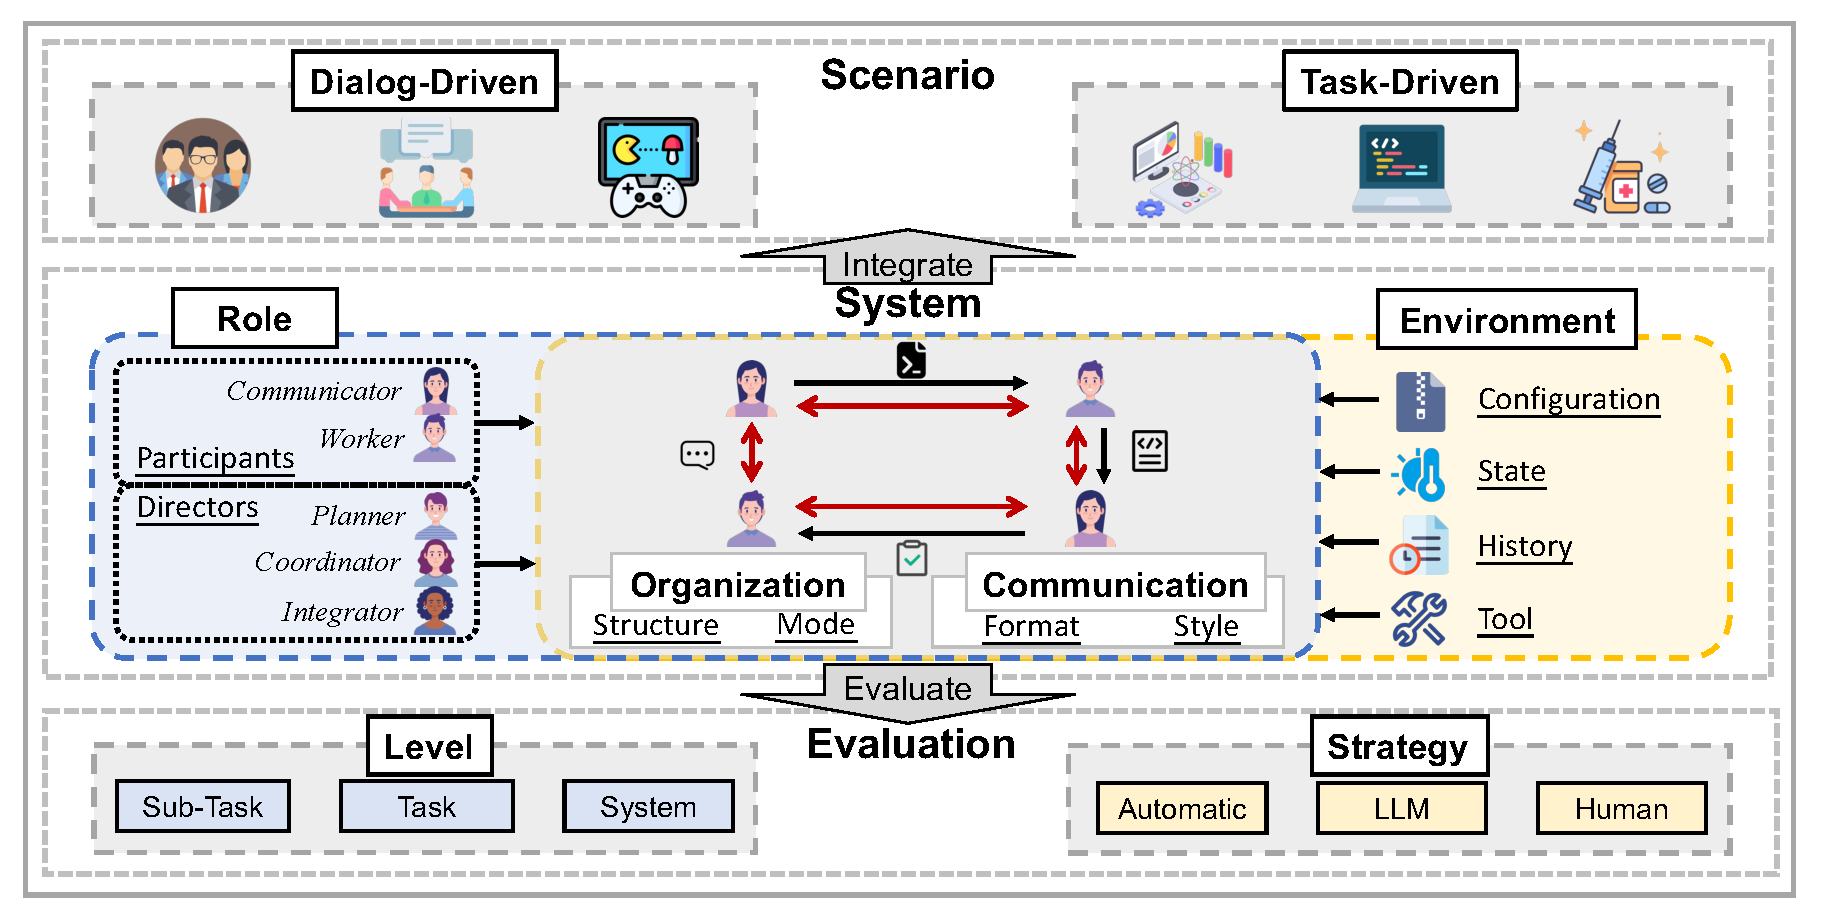
\includegraphics[width=\linewidth]{figs/fm_task_v2_3.pdf}
    \caption{Illustration of scenario simulations. Given a specific scenario, building a multi-agent {\ul system} involves modeling environment, roles, organization, and communication with detailed modules or mechanisms adjusted to the targeted scenario being supported. After simulating the {\ul scenario}, the desired output, typically the result of a task or problem, is obtained and {\ul evaluated} using different levels and strategies.}
    \label{fig:fm_task}
\end{figure*}

\subsection{Evaluation}\label{subsec:indi_eval}


To measure the performance of individual simulations, provide insights into their feasibility, and guide improvements to simulation architectures, researchers have developed diverse evaluation standards and methods, ranging from simple to complex approaches. These methods can be categorized into \textbf{static evaluation} and \textbf{interactive evaluation}.

\subsubsection{Static Evaluation}

Static evaluation refers to the dialogue-based assessment of LLMs by directly inducing their generation and measuring their quality. It can be categorized into subjective evaluation, which involves assessments by both LLMs and human evaluators, and objective evaluation, which utilizes mathematical tools for analysis.

\paragraph{Subjective Evaluation} Subjective evaluation refers to assessments conducted by humans or LLMs based on subjective standards. It often involves leveraging conversations with varying forms and contexts. Interview techniques are widely adopted~\cite{wang2024rolellmbenchmarkingelicitingenhancing,wang2024incharacterevaluatingpersonalityfidelity} because they can effectively prompt LLMs to generate expected responses. Other approaches, such as utterance imitation~\cite{deshpande2023toxicitychatgptanalyzingpersonaassigned}, are also favored in some research. Once dialogues are generated, some studies utilize advanced LLMs to evaluate the output on a given scale~\cite{wang2024incharacterevaluatingpersonalityfidelity,li2024personalllmagentsinsights,yu2024neekoleveragingdynamiclora}, considering performance dimensions. These dimensions range from psychology-based metrics, such as the Big Five Personality Traits (BFI) and Myers-Briggs Type Indicator (MBTI), to language-based factors like grammar and tone. Human annotators are often involved in experiments to provide human reference points ~\cite{park2023generativeagentsinteractivesimulacra,abbasian2024conversationalhealthagentspersonalized,baek2024knowledgeaugmentedlargelanguagemodels}.
\par
\paragraph{Objective Evaluation}Objective evaluation refers to assessments based on objective indicators, utilizing mathematical and statistical tools. It takes advantage of mathematical tools to grade the generation of simulating LLMs. Examination commonly involves option choosing(or questionnaire)~\cite{karra2023estimatingpersonalitywhiteboxlanguage}, ranking~\cite{gao2023livechatlargescalepersonalizeddialogue} and question answering~\cite{jang2022customizedconversationcustomizedconversation}. Accuracy~\cite{xiang2023languagemodelsmeetworld,li2024steerabilitylargelanguagemodels}, F1 score, recall~\cite{branch2022evaluatingsusceptibilitypretrainedlanguage,ahn-etal-2023-mpchat} are used in option choosing and ranking. In the examination of generation(question answering), text sequence related tools such as perplexity~\cite{li2016personabasedneuralconversationmodel,cho2022personalizeddialoguegeneratorimplicit,agrawal-etal-2023-multimodal}, ROUGE-L~\cite{Liu_2022,chen2023largelanguagemodelsmeet,xiang2023languagemodelsmeetworld} and BLUE~\cite{li2016personabasedneuralconversationmodel,Liu_2022,branch2022evaluatingsusceptibilitypretrainedlanguage,gao2023livechatlargescalepersonalizeddialogue} are broadly used in the evaluation, especially those with a reference version~\cite{chen2023largelanguagemodelsmeet}. Objective Examination is a more credible method of evaluating the performance of LLMs in individual simulation. However, it is highly restricted, and occasionally, specific objective tools must be developed to facilitate the evaluation of simulation in given dimensions.

\subsubsection{Interactive Evaluation}

Interactive evaluation refers to a circumstance-based assessment that creates a detailed interactive environment to measure the ability of individual simulations in complex scenarios. It is commonly applied in areas such as game performance~\cite{chalamalasetti2023clembenchusinggameplay,light2023avalonbenchevaluatingllmsplaying}, task completion~\cite{chen2023chatcottoolaugmentedchainofthoughtreasoning,wang2023chatcoderchatbasedrefinerequirement,farn2023tooltalkevaluatingtoolusageconversational}, and nuanced role-playing~\cite{chawla2023selfishwiselyinvestigatingimpact,jandaghi2023faithfulpersonabasedconversationaldataset}. Three key features of interactive evaluation are the carefully designed environment, real-time interactive external responses, and multi-stage assessments. Information about the crafted environment has been introduced in \S\ref{sec:action}. Real-time interactive external responses refer to the feedback from the external environment in reaction to the outputs of simulating LLMs. Agent-environment interactions construct multiple dialogues between the LLMs and the environment. These interactions help reveal the LLMs' capabilities in complex contexts, leading to more dynamic simulations. Single-aspect measurements are insufficient for interactive evaluation, so many studies adopt evaluated objectives that range from specific actions to hybrid actions~\cite{wang2024surveyagentconversationalpersonalizedefficient}, or from single-turn interactions to multi-turn dialogues~\cite{shao2023characterllmtrainableagentroleplaying}. Other studies assess generation quality, focusing on aspects such as accuracy relative to ground truth, nuanced simulations like tone imitation~\cite{wang2024rolellmbenchmarkingelicitingenhancing,huang2024embodiedgeneralistagent3d}, and self-reporting consistency~\cite{liu2023agentbenchevaluatingllmsagents}. In interactive evaluation, researchers prioritize not only accuracy but also the degree to which the simulation resembles real-world scenarios.

